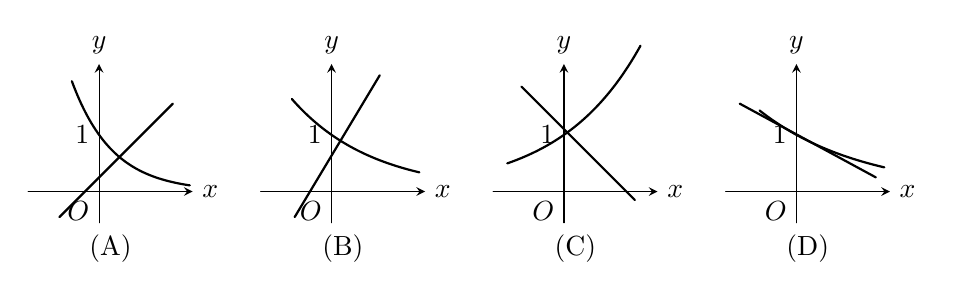
\begin{tikzpicture}[>=stealth,scale=0.72,line cap=round,line join=round]
\foreach \x/\name in {0/A,4.1/B,8.2/C,12.3/D}{
  \begin{scope}[shift={(\x,0)}]
    \draw[->] (-1.25,0)--(1.65,0) node[right] {$x$};
    \draw[->] (0,-0.55)--(0,2.25) node[above] {$y$};
    \node[left] at (0,1) {$1$};
    \node[below left] at (0,0) {$O$};
    \node at (0.2,-1.0) {(\name)};
  \end{scope}
}
% A: a>0 and 0<b<1; both curves use the same a,b.
\begin{scope}[shift={(0,0)}]
  \draw[thick,domain=-0.48:1.6,samples=80] plot (\x,{0.25^\x});
  \draw[thick] (-0.7,-0.45)--(1.3,1.55);
\end{scope}
% Distractor sketches retain the qualitative alternatives printed in the source.
\begin{scope}[shift={(4.1,0)}]
  \draw[thick,domain=-0.7:1.55,samples=80] plot (\x,{exp(-0.7*\x)});
  \draw[thick] (-0.65,-0.45)--(0.85,2.05);
\end{scope}
\begin{scope}[shift={(8.2,0)}]
  \draw[thick,domain=-1.0:1.35,samples=80] plot (\x,{exp(0.7*\x)});
  \draw[thick] (-0.75,1.85)--(1.25,-0.15);
\end{scope}
\begin{scope}[shift={(12.3,0)}]
  \draw[thick,domain=-0.65:1.55,samples=80] plot (\x,{exp(-0.55*\x)});
  \draw[thick] (-1.0,1.55)--(1.4,0.25);
\end{scope}
\end{tikzpicture}
